\begin{figure}[h!]
	\centering
	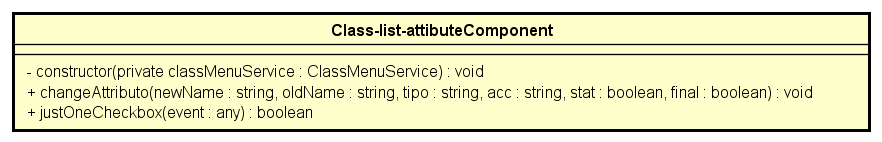
\includegraphics[scale=0.8]{res/sections/SpecificaFrontEnd/Components/Disegnetti/class-list-attribute.png}
	\caption{Diagramma della classe Class-list-attribute}
\end{figure}

\begin{figure}[h!]
	\centering
	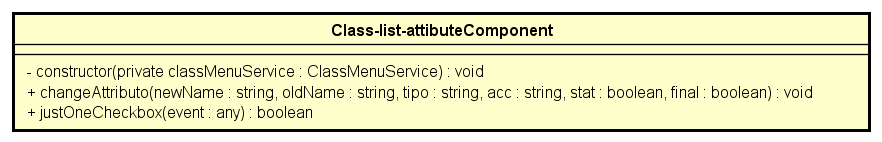
\includegraphics[scale=0.8]{res/sections/SpecificaFrontEnd/Components/Disegnetti/class-list-attribute.png}
	\caption{Diagramma della classe Class-list-attribute}
\end{figure}

\begin{itemize}
	\item \textbf{Descrizione:}\\
	
	\item \textbf{Utilizzo:}\\
	
	\item \textbf{Metodi:}
		\begin{itemize}
			\item \emph{-constructor(private classMenuService: ClassMenuService)}\\
    		Costruttore della classe\\
    		\textbf{Parametri:}
    		\begin{itemize}
    			\item \emph{classMenuService: ClassMenuService}\\
    			Crea un istanziazione di ClassMenuService
    		\end{itemize}
    		\item \emph{+changeAttributo(newName: string, oldName: string, tipo: string, acc: string, stat: boolean, final: boolean)}\\
    		Modifica le proprietà di un attributo\\
    		\textbf{Parametri:}
    		\begin{itemize}
    			\item \emph{newName: string}\\
    			Nuovo nome dell'attributo
    			\item \emph{oldName: string}\\
    			Vecchio nome dell'attributo
    			\item \emph{tipo: string}\\
    			Tipo dell'attributo
    			\item \emph{acc: string}\\
    			Visibilità dell'attributo
    			\item \emph{stat: boolean}\\
    			True se è marcato static
    			\item \emph{final: boolean}\\
    			True se è marcato final
    		\end{itemize}
    		\item \emph{+justOneCheckbox(event: any)}\\
    		Controlla che ci sia solo un elemento sulla checkbox\\
    		\textbf{Parametri:}
    		\begin{itemize}
    			\item \emph{event: any}\\
    			Nome dell'elemento
    		\end{itemize}
		\end{itemize}
\end{itemize}